% !TeX spellcheck = es_MX-SpanishMexico
%----------------------------------------------------------------------------------------------------
%                           		  ENTRE LÍNEAS DE TIERRA

% Curso: Arqueología Bíblica
% Módulo 1: Introducción, Definiciones y Conceptos
% Elabora: Rodrigo Gerardo Trejo Arriaga

%----------------------------------------------------------------------------------------------------

% FORMATO DEL DOCUMENTO


\documentclass[11pt]{article} % Letra estandar

\usepackage[utf8]{inputenc}

%\usepackage{tgadventor}
%\renewcommand{\familydefault}{\sfdefault}

\usepackage[light,math]{iwona}

\usepackage[T1]{fontenc}


\usepackage[spanish]{babel}
\addto\captionsspanish{\renewcommand{\abstractname}{\large{Introducción}}}

\usepackage[margin=1in,letterpaper]{geometry}

\usepackage{fancyhdr} % Paquete para personalizar encabezado y pie de página
\pagestyle{fancy} % Establece que personalizaremos el pie de pagina y el encabezado
\setlength{\headheight}{13.59999pt} % Establece la altura del encabezado
\fancyhead[R]{\textcolor{darkBlue}{Teoría de la Computación}} % Encabezado derecho
\fancyhead[L]{\textit{\textcolor{darkBlue}{Escuela Superior de Cómputo}}} % Encabezado izquierdo
\fancyfoot[L]{\textit{\textcolor{darkBlue}{Práctica 1}}} % Pie de página izquierdo 
\fancyfoot[R]{\textcolor{darkBlue}{\thepage}} % Pie de página  derecho
\fancyfoot[C]{} % Elimina la nueración central de páginas en el pie de página
\renewcommand{\headrulewidth}{0.5pt} % Grosor de la linea de encabezado
\renewcommand{\footrulewidth}{0.5pt} % Grosor de la linea de pie de página

\usepackage{enumitem}

\usepackage{changepage}

\usepackage{graphicx}

\usepackage{tabularx}

\setlength{\parskip}{8pt}

\usepackage{xcolor}
\definecolor{darkBlue}{rgb}{0,0,0.31}
%\definecolor{darkBlue}{rgb}{0,0,0.5}
\definecolor{munsell}{rgb}{0.0, 0.5, 0.69}
\definecolor{indigo}{rgb}{0.0, 0.25, 0.42}
\renewcommand{\footrulewidth}{2pt}
\renewcommand{\footrule}{\hbox to\headwidth{\color{darkBlue}\leaders\hrule height \footrulewidth\hfill}}

\usepackage{colortbl}

\usepackage{titlesec}
\titleformat{\section}
{\normalfont\Large\bfseries\color{darkBlue}}{\thesection.}{1em}{}

\usepackage{tabularx}

\usepackage{textcomp}

\usepackage{titling}

\usepackage{apacite}
\bibliographystyle{apacite}

%\usepackage{natbib}
%\setlength{\bibsep}{6pt}

\usepackage{setspace}

\usepackage{listings}


\lstset{
	language=Python,                % Lenguaje del código (Python en este caso)
	basicstyle=\ttfamily,           % Estilo de fuente
	keywordstyle=\color{blue},      % Estilo para las palabras clave
	commentstyle=\color{green},     % Estilo para los comentarios
	numbers=left,                   % Colocar números de línea a la izquierda
	numberstyle=\tiny\color{gray},  % Estilo para los números de línea
	stepnumber=1,                   % Número de línea cada 1 línea
	tabsize=4,                      % Tamaño de la tabulación
	frame=single,                   % Colocar un marco alrededor del código
	breaklines=true,                % Romper líneas largas automáticamente
	showstringspaces=false,         % No mostrar espacios en cadenas
	escapeinside={(*@}{@*)},        % Para incluir caracteres especiales en el código
	extendedchars=true               % Permitir caracteres especiales, como acentos
}


\renewcommand{\thesection}{\Roman{section}}

%----------------------------------------------------------------------------------------------------
% CUERPO DEL DOCUMENTO

\begin{document}
	
	\begin{titlepage}
		\centering
		{
\includegraphics[width=0.25\textwidth]{descarga}\par}
		\vspace{0.5cm}
		{\bfseries\huge Escuela Superior de Cómputo \par}
		\vspace{0.7cm}
		{\scshape\LARGE Teoría de la Computación \par}
		\vspace{0.3cm}
		\vspace{3.1cm}
		{\scshape \Huge \textbf{Práctica 1:}  \par}
		\vspace{0.03cm}
		{{\LARGE \textit{Universo}} \par}
		%\vfill
		\vspace{3.5cm}
		{\Large Autor: \par}
		{\Large Rodrigo Gerardo Trejo Arriaga \par}
		%\vfill
		\vspace{3cm}
		{\Large Octubre 2023 \par}
	\end{titlepage}
	
	\begin{center}
		\vspace*{0.1cm}
		{\huge \textcolor{darkBlue}{\textbf{Práctica 1:}} \par}
		
		{\Large \textcolor{darkBlue}{\textbf{\textit{Universo}}}}
	\end{center}
	
	En la teoría de la computación, un alfabeto se define como un conjunto finito de símbolos o caracteres. Estos símbolos son la base fundamental para construir cadenas o secuencias de símbolos. Por ejemplo, en el contexto de la teoría de la computación, es común utilizar el alfabeto ${0, 1}$ para representar símbolos binarios.
	
	Una cadena, también conocida como palabra, es una secuencia finita de símbolos tomados de un alfabeto dado. Estas cadenas desempeñan un papel esencial en la representación de datos y forman la base de los lenguajes formales en la teoría de la computación.
	
	El conjunto universo, por otro lado, hace referencia a un conjunto que contiene todos los objetos posibles que son relevantes para un problema o lenguaje específico. Por ejemplo, si se trata de un lenguaje de programación, el conjunto universo podría consistir en todos los programas concebibles que se pueden escribir en ese lenguaje.
	
	En el contexto de la teoría de la computación, un lenguaje formal se define como un conjunto de cadenas (palabras) construidas a partir de un alfabeto dado. Estos lenguajes formales se utilizan para describir propiedades de las cadenas y son fundamentales en la definición de gramáticas formales, autómatas y en la resolución de diversos problemas relacionados con la informática teórica.
	
	En esta práctica presentaremos un programa que conjunta todos estos conceptos.
	
	\section{Descripción del problema}
	
	Este programa calcula el universo de cadenas binarias ($\Sigma^n$), donde "n" es un valor determinado por el usuario o calculado automáticamente por el programa. El rango de "n" está restringido al intervalo [0, 1000].
	
	\begin{enumerate}
		\item Ejecute el programa y especifique el valor de "n" que desea calcular.
		\item El programa preguntará si desea calcular otro valor de "n" o salir.
		\item Los resultados se guardarán en un archivo de texto en notación de conjunto.
		\item A continuación, graficaremos el número de unos en cada cadena. El eje "x" representa las cadenas y el eje "y" representa el número de unos en cada cadena.
		\item En el informe, se explicará, calculará y graficará el caso específico en el que "n=28".
		\item Además, se calculará una segunda gráfica utilizando el logaritmo en base 10 del número de unos.
	\end{enumerate}
	
	
	\section{Resultados}
	

	
	\begin{figure}[h]
		\centering
		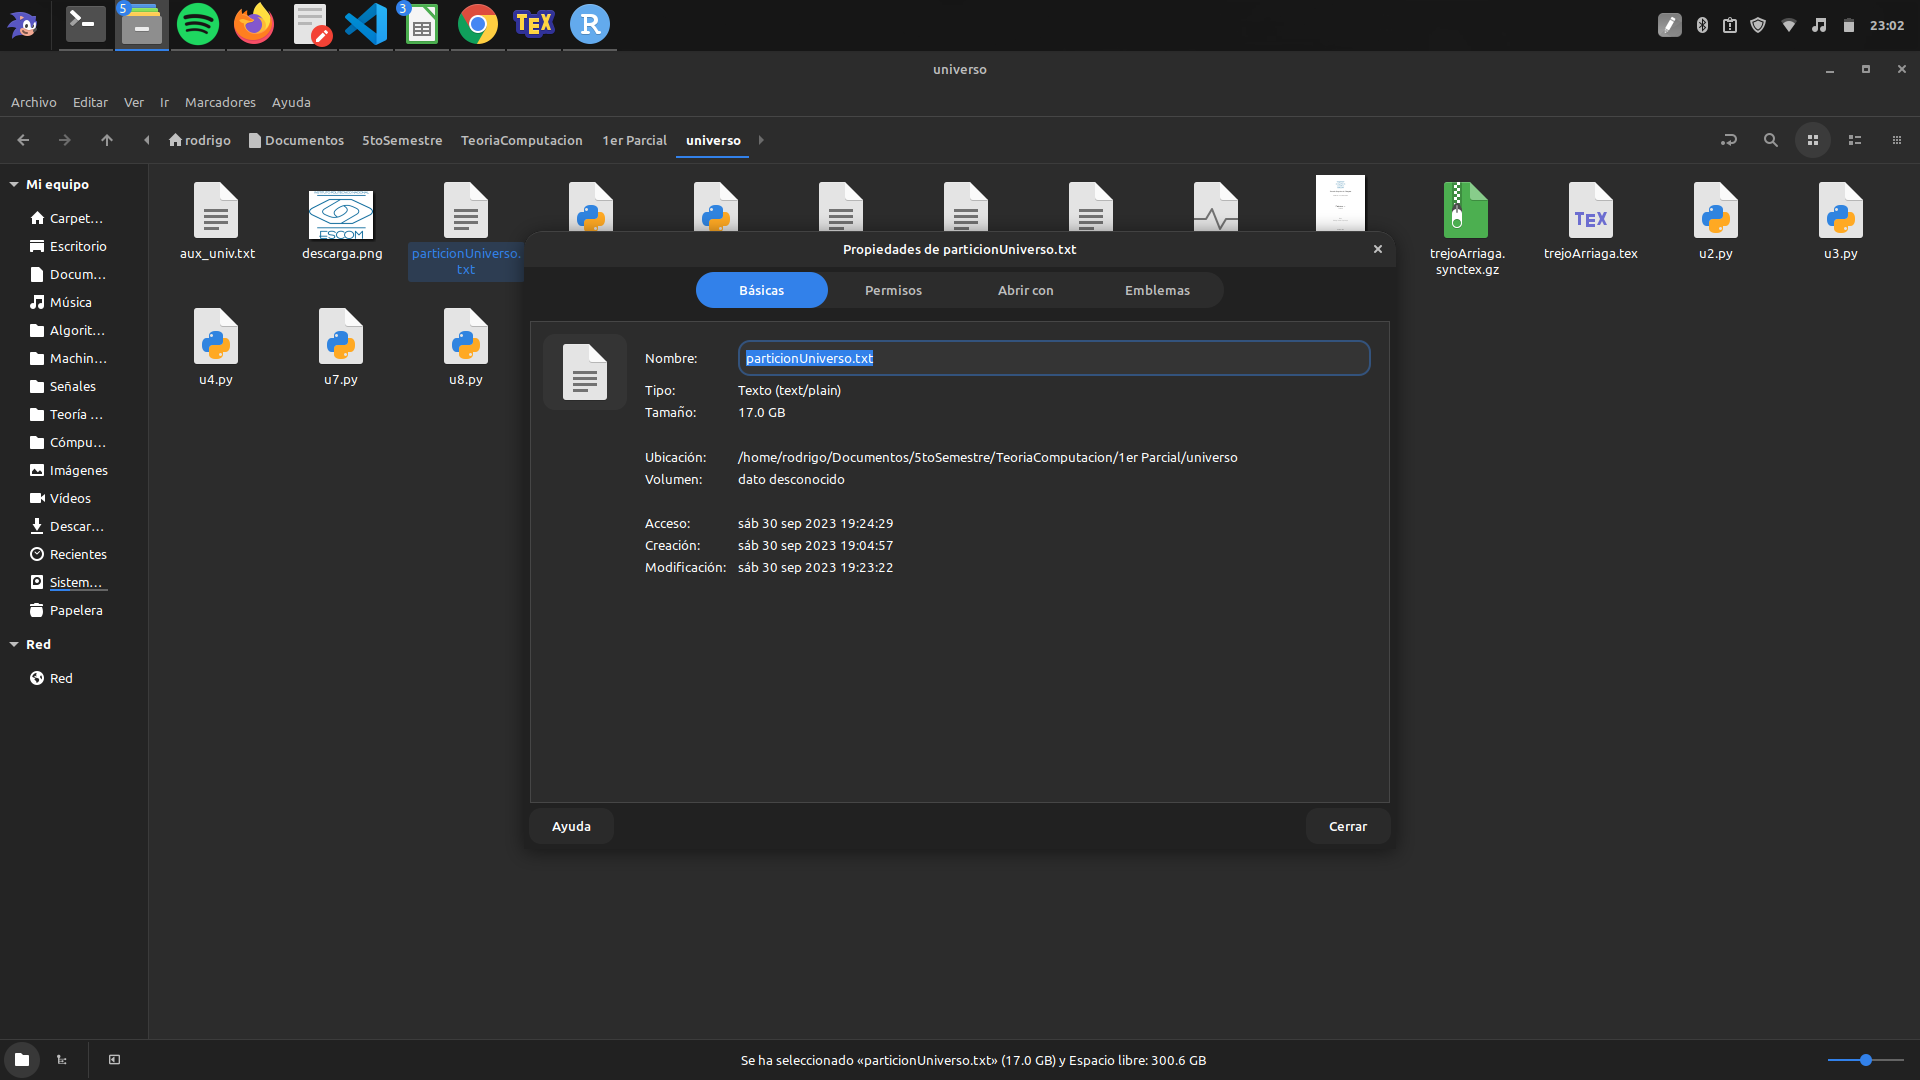
\includegraphics[width=0.8\textwidth]{imagen1u.png}
		\caption{Gráfica de numero vs num de unos}
	\end{figure}
	
	\begin{figure}[h]
		\centering
		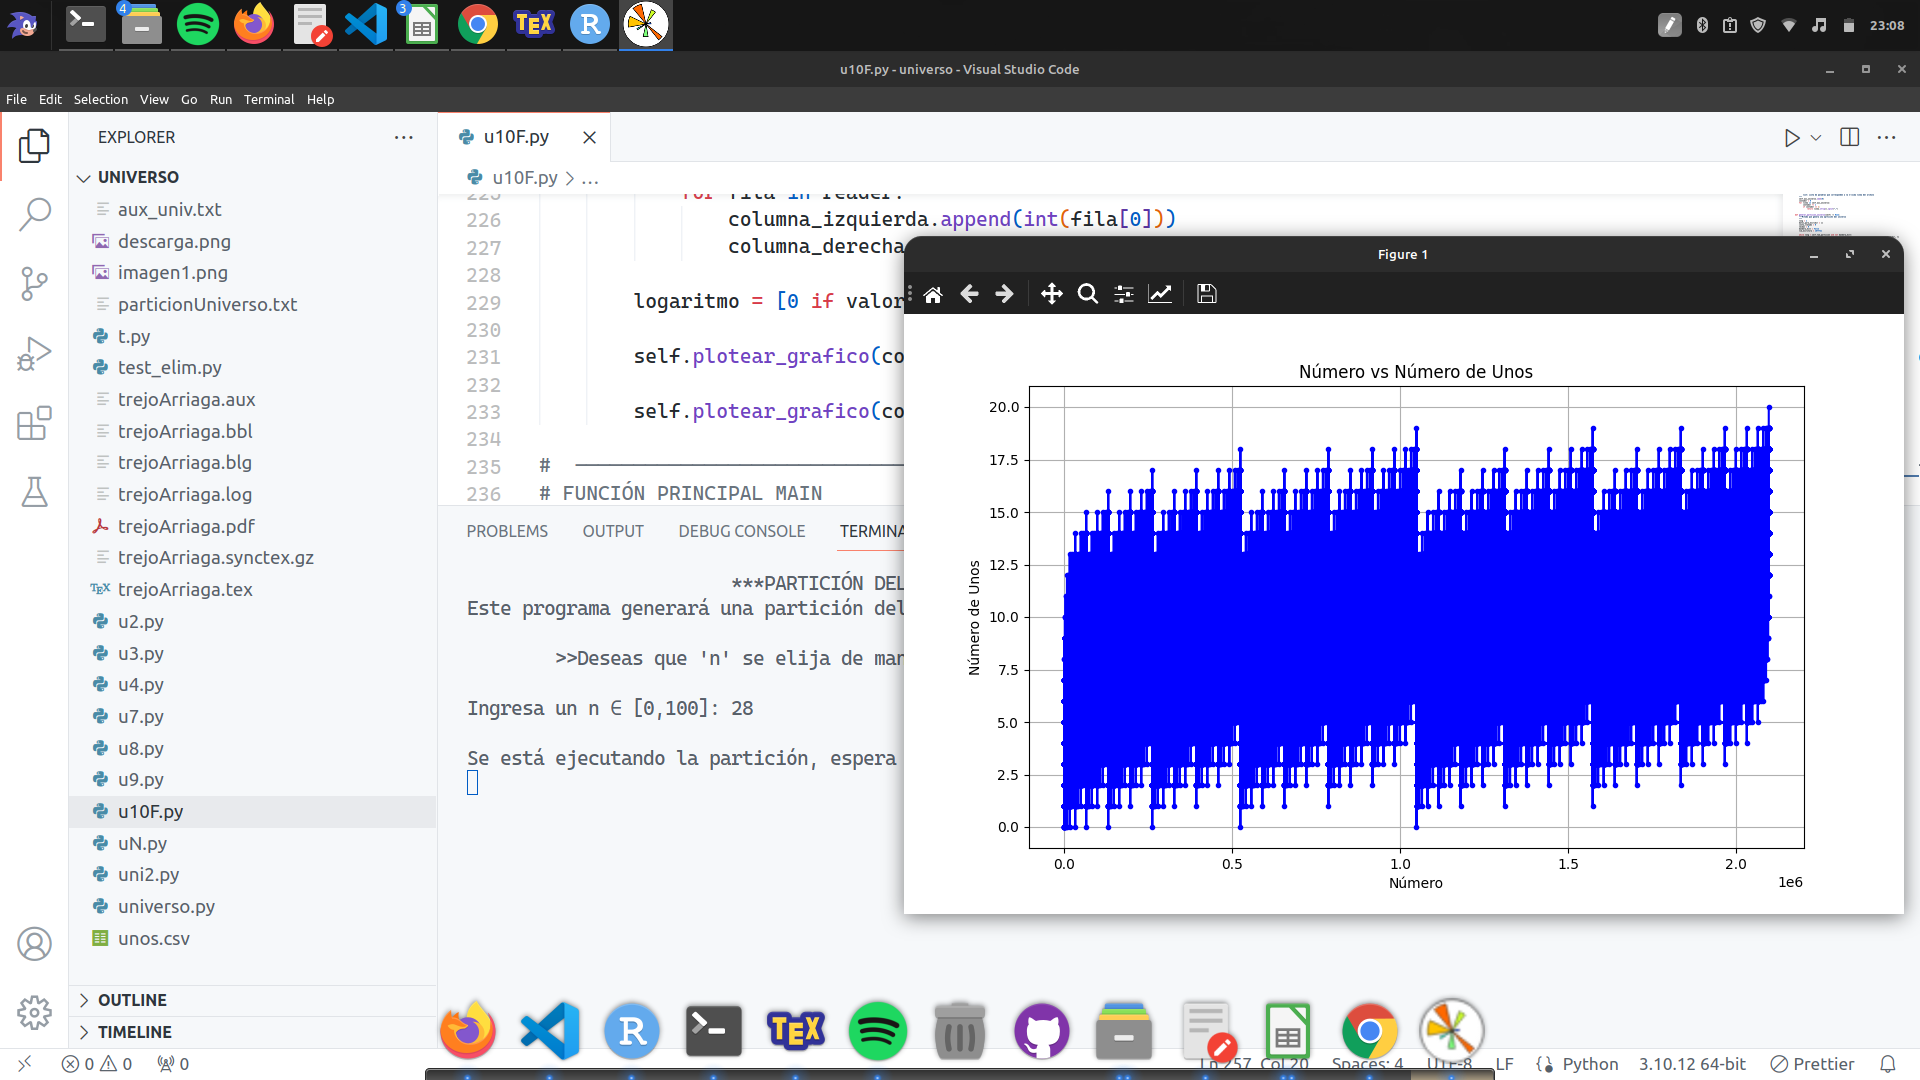
\includegraphics[width=0.8\textwidth]{imagen2u.png}
		\caption{}
	\end{figure}
	
	\begin{figure}[h]
		\centering
		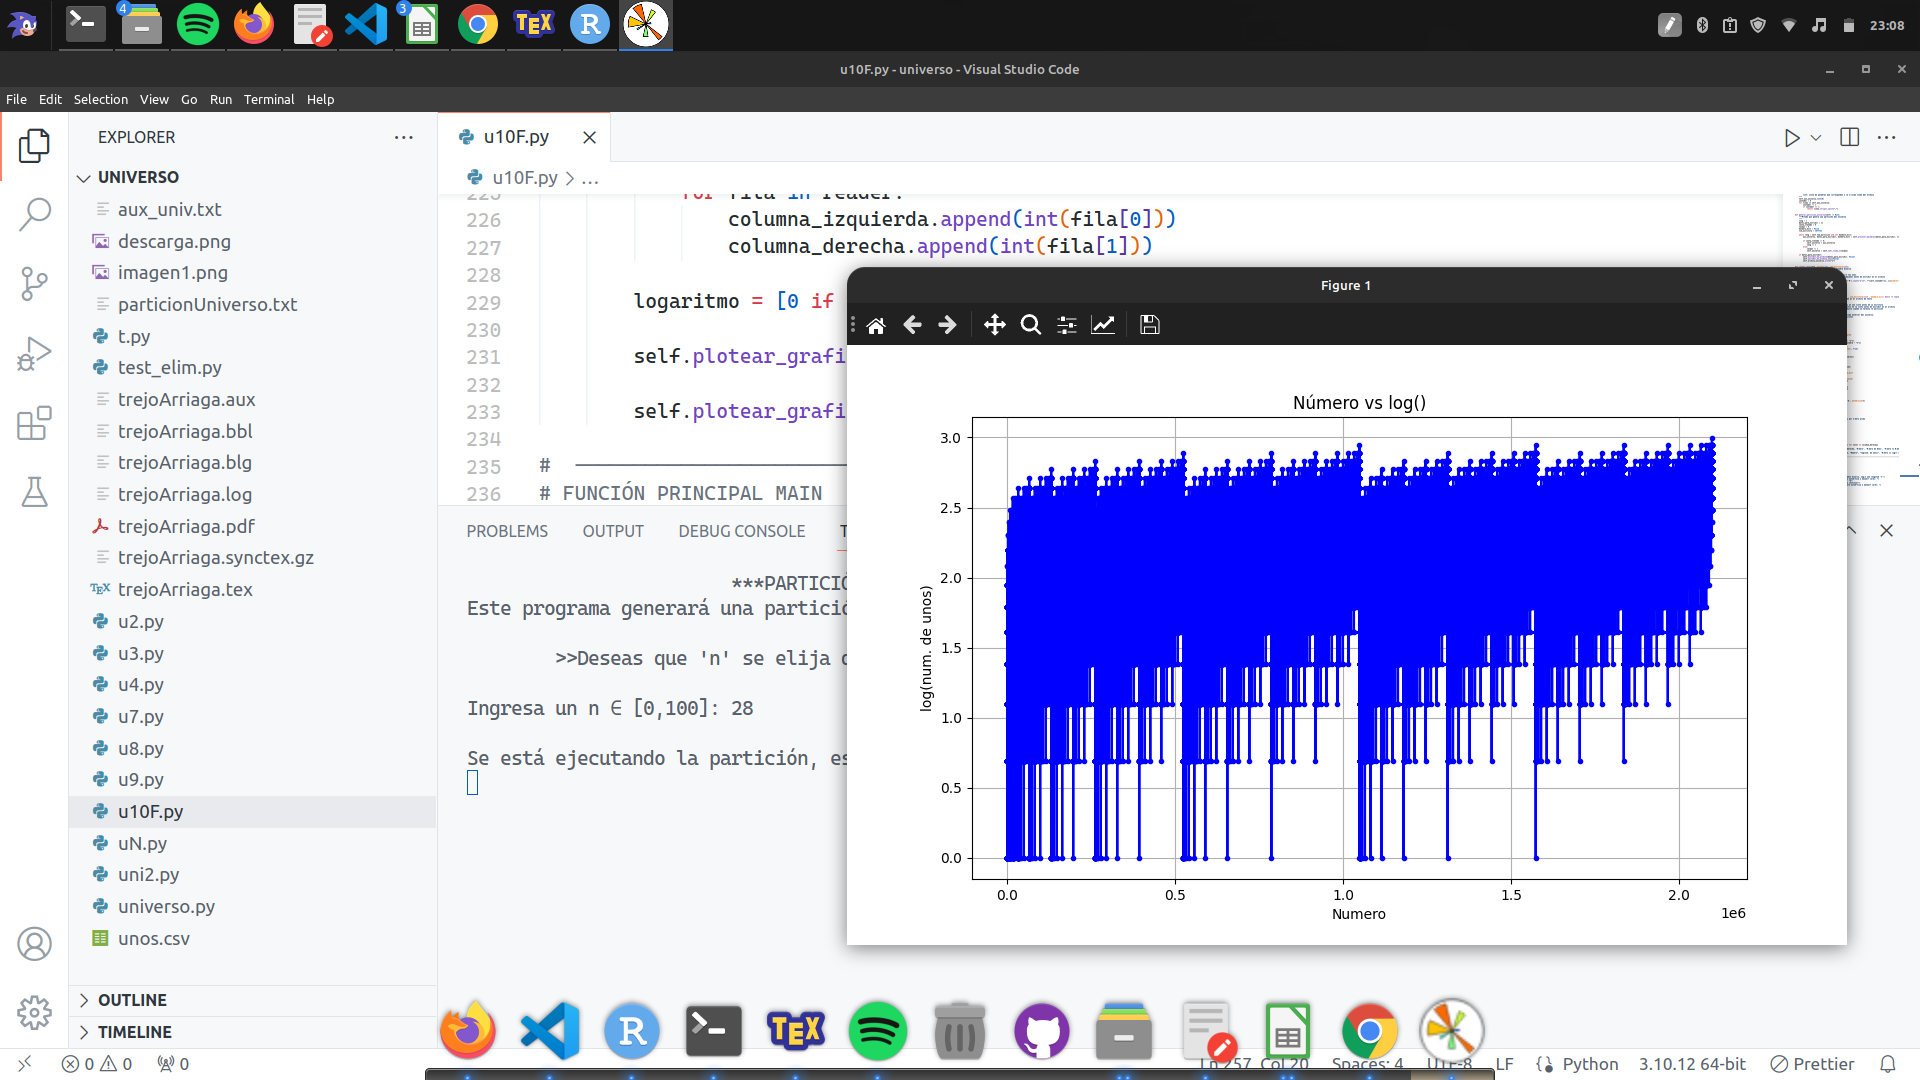
\includegraphics[width=0.8\textwidth]{imagen3u.png}
		\caption{Gráfica Logaritmo}
	\end{figure}
	
	
	\section{Código de Implementación}
	
		\begin{lstlisting}
		'''
		INSTITUTO POLITÉCNICO NACIONAL
		ESCUELA SUPERIOR DE CÓMPUTO
		
		INGENIERÍA EN INTELIGENCIA ARTIFICIAL
		
		TEORÍA DE LA COMPUTACIÓN
		PARTICIÓN DEL UNIVERSO DE PALABRAS BINARIAS
		
		GRUPO: 5BM1
		ALUMNO: TREJO ARRIAGA RODRIGO GERARDO
		
		ESTE PROGRAMA GENERA UNA PARTICIÓN DEL UNIVERSO DE PALABRAS BINARIAS:
		i) ESCRIBE LA PARTICIÓN EN UN ARCHIVO DE TEXTO
		ii) GENERA UNA GRÁFICA DE LAS PALABRAS BINARIAS VS EL NÚMERO DE UNOS QUE TIENEN
		iii) GENERA UNA GRÁFICA DE LAS PALABRAS BINARIAS VS EL LOGARITMO DEL NÚMERO DE UNOS
		PARA APRECIAR MEJOR SU CRECIMIENTO
		
		ÚLTIMA MODIFICACIÓN: 13/10/2023
		'''
		
		#  --------------------------------------------------------------------------------------------------------------------
		# MÓDULOS Y LIBRERÍAS IMPORTADAS
		
		
		import os
		import time
		import random
		import matplotlib.pyplot as plt
		import csv
		import math
		
		#  --------------------------------------------------------------------------------------------------------------------
		# FUNCIONES
		
		
		def eliminar_archs(nombre_arch):
		"""Función que elimina un archivo si existe en el directorio
		
		Args:
		nombre_arch (str): Nombre del archivo que deseas eliminar
		"""
		archivo1 = nombre_arch
		if os.path.exists(archivo1):
		os.remove(archivo1)
		
		#  --------------------------------------------------------------------------------------------------------------------
		# CLASES
		
		
		class ParticionUniverso:
		
		def __init__(self, tam_particion: int, nombre_arch="particionUniverso", nombre_aux="aux_univ.txt") -> None:
		"""Constructor de la clase que hace la partición del universo
		
		Args:
		tam_particion (int): Tamaño de la particion que se desea reaizar
		nombre_arch (str, optional): Nombre del archivo donde se almacena la particion de longitud especificada. Defaults to "particionUniverso".
		nombre_aux (str, optional): Archivo que sirve como auxiliar de las particiones. Defaults to "aux_univ.txt".
		"""
		self.nombre_arch = nombre_arch
		self.tam_particion = tam_particion
		self.universo = ["0", "1"]
		self.archivo_universo = open(f"{nombre_arch}.txt", "a+", encoding="utf-8")
		self.archivo_universo.write("Σ = {ε, 0, 1, ")
			self.aux_universo = open(nombre_aux, "a+", encoding="utf-8")
			self.contador = 2
			self.unos = ["1, 0", "2, 1"]
			self.num_palabra = [1, 2]
			self.arch_num_unos = open("unos.csv", "a+", encoding="utf-8")
			
			
			def escribir_en_archivo(self, datos:list, escribir_coma: bool)-> None:
			"""Método que escribe datos en el archivo de particion de universo
			
			Args:
			datos (list): Datos pertenecientes a la partición
			escribir_coma (bool): Bandera para escribir coma al final del uktimo caracter
			"""
			self.archivo_universo.write(", ".join(datos))
			if escribir_coma:
			self.archivo_universo.write(", ")
			
			
			def escribir_en_archivo_unos(self, escribir_salto: bool)-> None:
			"""Método que escribe datos en el archivo de particion de universo
			
			Args:
			datos (list): Datos pertenecientes a la partición
			escribir_coma (bool): Bandera para escribir coma al final del uktimo caracter
			"""
			self.arch_num_unos.write("\n".join(self.unos))
			if escribir_salto:
			self.arch_num_unos.write("\n")
			
			
			def leer_linea_n(self, n:int) -> list:
			"""Método que lee la linea n-ésima de un archivo
			
			Args:
			n (int): Número de linea que se desea leer
			
			Returns:
			list: Lista de palabras que corresponden a la n-ésima linea del archuvo
			"""
			self.aux_universo.seek(0)
			contador = 0
			for linea in self.aux_universo:
			contador += 1
			if contador == n:
			return linea.strip().split(",")
			
			
			def generar_particion_universo(self) -> None:
			"""Método que genera una aprtición del universo
			"""
			long = 1
			datos_para_escribir = []
			conta_llenado = 0
			leidas = 0
			bandera_kill = False
			lim_escritura = 1677721
			
			while long < self.tam_particion and not bandera_kill:
			aux_universo, datos_para_escribir, bandera_kill = self.procesar_palabras(datos_para_escribir, lim_escritura, bandera_kill)
			
			if conta_llenado == 0:
			self.universo = aux_universo
			long += 1
			else:
			leidas += 1
			self.universo = self.leer_linea_n(leidas)
			
			if datos_para_escribir:
			self.escribir_en_archivo(datos_para_escribir, False)
			self.escribir_en_archivo_unos(False)
			self.archivo_universo.write("}")
		
		
		def contar_unos(self, palabra:str, cte_escritura:int):
		"""Método que cuenta los unos en una palabra binaria
		
		Args:
		palabra (str): Palabra de la que se contarán los unos
		cte_escritura (int): límite de cadenas a almacenar antes de escribir en el archivo 
		"""
		self.unos.extend([f"{self.contador+1}, {(palabra+'0').count('1')}", f"{self.contador+2}, {(palabra+'1').count('1')}"])
		self.contador += 2
		
		if len(self.unos) > cte_escritura:
		self.escribir_en_archivo_unos(True)
		self.unos = []
		
		
		def procesar_palabras(self, datos_para_escribir:list , lim_escritura:list , bandera_kill: bool) -> tuple:
		"""Método que genera nuevas palabras y las escribe en el archivo de texto
		
		Args:
		datos_para_escribir (list): Datos almacenados en una lista antes de su escritura
		lim_escritura (list): Número máximo de elementos en la lista antes de escribir en el archivo
		bandera_kill (bool): Bandera que termina el bucle cuando se termina la partición
		
		Returns:
		tuple: Tupla con la lista auxiliar de la corrida anterior del universo,
		la lista de datos que esperan ser escritos 
		y la bandera de término de ciclo
		"""
		aux_universo = []
		conta_llenado = 0
		for palabra in self.universo:
		
		if self.tam_particion == 28:
		if (self.contador+2) % 1000:
		self.contar_unos(palabra, lim_escritura)
		else:
		self.contar_unos(palabra, lim_escritura)
		aux_universo.extend([palabra + "0", palabra + "1"])
		datos_para_escribir.extend([palabra + "0", palabra + "1"])
		
		if len(datos_para_escribir) >= lim_escritura:
		self.escribir_en_archivo(datos_para_escribir, True)
		datos_para_escribir = []
		
		if len(aux_universo) == lim_escritura:
		self.aux_universo.write(",".join(aux_universo))
		self.aux_universo.write("\n")
		conta_llenado += 1
		aux_universo = []
		
		if palabra.count("1") + 1 == self.tam_particion:
		bandera_kill = True
		
		return aux_universo, datos_para_escribir, bandera_kill
		
		
		def plotear_grafico(self, x, y, label_x, label_y, titulo):
		"""Método que plotea una gráfica según dos listas
		
		Args:
		x (list): Lista de datos que irán en el eje x 
		y (list): Lista de datos que irán en el eje y
		titulo (str): Título de la gráfica
		label_x (str): Etiqueta del eje x
		label_y (str): Etiqueta del eje y
		"""
		plt.figure(figsize=(10, 6))
		plt.plot(x, y, marker='o', linestyle='-', color='b', markersize=3)
		plt.title(titulo)
		plt.xlabel(label_x)
		plt.ylabel(label_y)
		plt.grid(True)
		plt.show()
		
		
		def graficar_num_unos(self):
		"""Función que hace la gráfica del número de unos por número primo
		"""
		columna_izquierda = []
		columna_derecha = []
		
		with open("unos.csv", 'r+') as archivo_csv:
		reader = csv.reader(archivo_csv)
		
		
		for fila in reader:
		columna_izquierda.append(int(fila[0]))
		columna_derecha.append(int(fila[1]))
		
		logaritmo = [0 if valor == 0 else math.log(valor) for valor in columna_derecha]
		
		self.plotear_grafico(columna_izquierda, columna_derecha, 'Número', 'Número de Unos', 'Número vs Número de Unos')
		
		self.plotear_grafico(columna_izquierda, logaritmo, "Numero", "log(num. de unos)", 'Número vs log()')
		
		#  --------------------------------------------------------------------------------------------------------------------
		# FUNCIÓN PRINCIPAL MAIN
		
		
		if __name__ == "__main__":
		os.system('clear')
		eliminar_archs("particionUniverso.txt")
		eliminar_archs("aux_univ.txt")
		eliminar_archs("unos.csv")
		print("\t\t\t***PARTICIÓN DEL UNIVERSO***")
		print("Este programa generará una partición del alfabeto binario, según una longitud 'n'")
		modo = input("\n\t>>Deseas que 'n' se elija de manera automática o manual? [a/m]: ")
		while not modo.lower() != "a" and not modo.lower() != "m":
		print("Modo inválido, ingreséselo nuevamente para continuar")
		modo = input("\t>>Deseas que 'n' se elija de manera automática o manual? [a/m]: ")
		
		match modo:
		case "a":
		n = random.randint(0, 28)
		print(f"\nSe ha elegido un n={n}")
		case _:
		n = int(input("\nIngresa un n ∈ [0,100]: "))
		
		print("\nSe está ejecutando la partición, espera un momento.")
		inicio = time.perf_counter()
		test = ParticionUniverso(n)
		test.generar_particion_universo()
		fin = time.perf_counter()
		tiempo_transcurrido = fin - inicio
		test.arch_num_unos.close()
		test.graficar_num_unos()
		eliminar_archs("aux_univ.txt")
		eliminar_archs("unos.csv")
		print("\nListo, puedes consultar la partición en el archivo: 'particionUniverso.txt'.")
		print(f"Tiempo de generacion de la particion: {tiempo_transcurrido:.5f} segundos")
		
	\end{lstlisting}
	
	

	
	
\end{document}